%%%%%%%%%%%%%%%%%%%%%%%%%%%%%%%%%%%%%%%%%%%%%%%%%%%%%%%%%%%%%%%%

% IEEEconf.cls file must exist in the same directory as the TeX file you want to compile
\documentclass[letterpaper, 10 pt, conference]{IEEEconf}

\title{\LARGE \bf
Computer History:\\Integrated Circuits
}
%why is the first email the only one that is small?
\author{Jordan Medina\\Kenji Helms\\Guillmer Germino\\
\small guillmer.germino@student.nmt.edu\\
\small kenji.helms@student.nmt.edu\\
\small jordan.medina@student.nmt.edu\\
\small {October 2020}
}

% Image/graphics support
\usepackage{graphicx} % takes care of graphic
\graphicspath{ {./images/} } %full file path to the images

% Formatting for lists
\usepackage{enumitem}

% Formatting for media
\usepackage{float}
\restylefloat{table}
\restylefloat{figure}
\usepackage[utf8]{inputenc}
\usepackage{epigraph}
\usepackage{graphicx}
\usepackage{caption}

\begin{document}


\maketitle




%%%%%%%%%%%%%%%%%%%%%%%%%%%%%%%%%%%%%%%%%%%%%%%%%%%%%%%%%%%%%%%%%%%%%%%%%%%%%%%%
\section{\underline{Introduction}\\\\
\small {\underline{The Confluence of Hardware and Software}}}

This document is a basic template for writing conference-style                  
reports in LaTeX. You will use this template when writing                       
your report; you will need to replace all text (excluding                       
section headers or preamble information) with the content                       
of your report.

\section{History}
Intro to the history here...

\subsection{Vacuum Tube Technology}
Talk about vacuum tubes

\begin{figure}[h!]
\centering
\captionsetup{justification=centering}
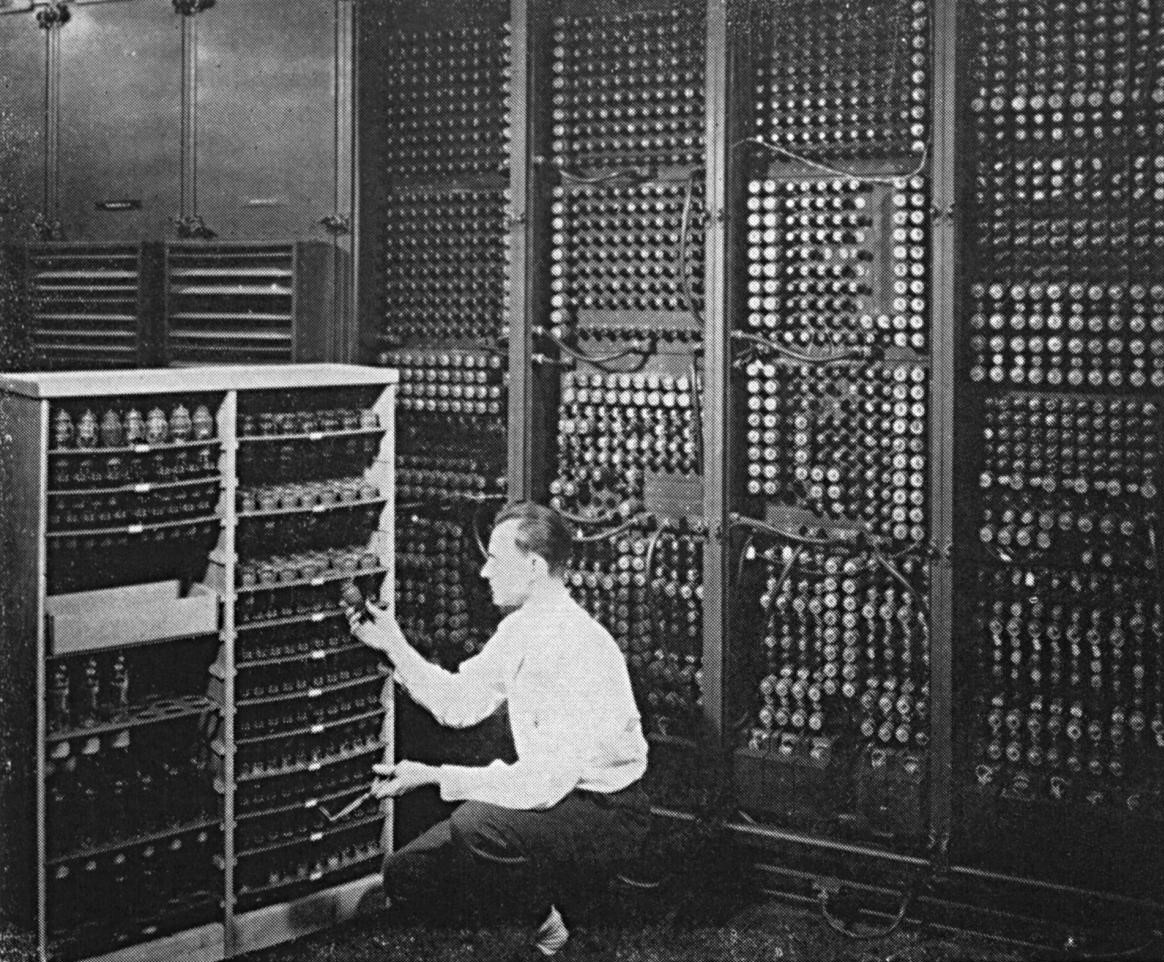
\includegraphics[width=0.2\textwidth]{ENIAC-changing_a_tube.jpg}
\caption{A technician changes a vacuum tube in the ENIAC}
\label{fig:example}
\end{figure} 



%Talk about the timeline from vacuum tube, 

\section{Theory}

Talk about the necessity of using circuits. Why are they needed at all? How do they accomplish the basic ideas from a model of information transfer/logic?


\section{Moore's Law}


\begin{figure}[h!]
\centering
\captionsetup{justification=centering}
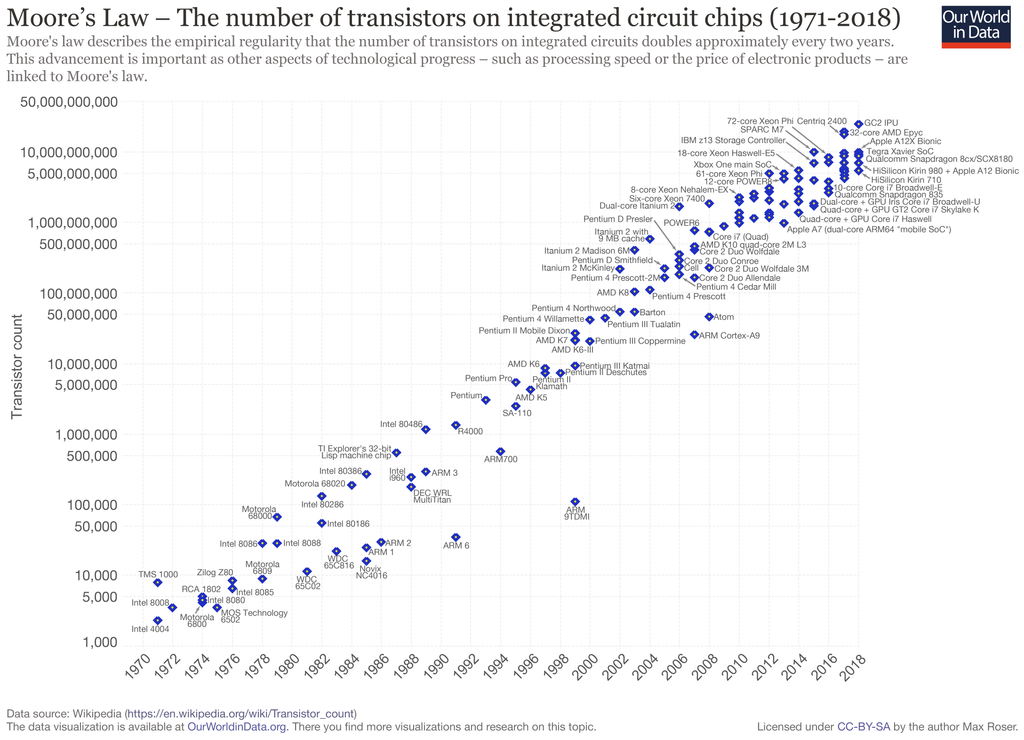
\includegraphics[width=0.2\textwidth]{1024px-Moore's_Law_Transistor_Count_1971-2018.png}
\caption{Integrated Circuit complexity over time, 1970-2018}
\label{fig:example}
\end{figure} 
Integrated Circuits have gone through an immense growth per physical size over the years, leading to many of the breakthroughs enjoyed in modern technology. Talk about how Moore's Law uses ICs as a metric of computer tech sophistication.


\section{Cost/Efficiency}



\section{CONCLUSION}

Conclude the ideas.

\section*{REFERENCES}


\begin{enumerate}[label={[\arabic*]}]
\item https://www.newegg.com/p/N82E16811112392
\item https://www.nvidia.com/en-us/geforce/graphics-cards/30-series/rtx-3080/
\item https://www.intel.com/content/www/us/en/products/processors/core/i9-processors/i9-10900.html
\item https://www.newegg.com/corsair-32gb-260-pin-ddr4-so-dimm/p/N82E16820236682
\item https://www.pcmag.com/reviews/acer-predator-x27
\item https://www.amazon.com/Toshiba-Performance-Desktop-Internal-HDWE150XZSTA/dp/B013JPLKQK
\end{enumerate}

\end{document}


